%!TEX root = ../main.tex

\thispagestyle{empty}
\vspace{-0.7cm}

\cleanchapterquote{Hasta el día de hoy, los matemáticos han intentado en vano descubrir algún orden en la secuencia de números primos, y tenemos razones para creer que es un misterio al que la mente humana nunca penetrará}{Leonhard Euler}{}

Para comenzar con este capítulo presentaremos el teorema fundamental de la aritmética (TFA), una pieza crucial en cualquier trabajo sobre teoría de números.\\


\begin{theorem}[TFA]
Todo entero $n>1$ se puede escribir como producto de primos de manera única salvo el orden de los factores, es decir:

$$n=\prod_{j=1}^{m}p_j^{k_j}$$
\end{theorem}

Escribiremos $p^m\mid\mid n$ siempre que si $p^m\mid n$ entonces $p^{m+1}\nmid n$, es decir, $p^m$ es la potencia exacta que divide a $n$, esto nos permite escribir el TFA como:

$$n= \prod_{p^m\mid\mid n}p^m$$

\section{Funciones aritmética}

\begin{definition}
Una función aritmética es una función con dominio los naturales y rango $\R$ o $\C$, es decir $a$ es función aritmética si:

$$f:\N \to \mathbb{F}$$

con $\mathbb{F}=\C$ o $\mathbb{F}=\R$
\end{definition}

Esta definición nos muestra que las funciones aritmética no son más que sucesiones de números reales o complejos, en algunos casos será útil considerarlas de esta  manera y de manera análoga a  las sucesiones las denotaremos como $a_n$, donde cada $a_n$ representa $f(n)$. Veamos algunos ejemplos importantes:

\begin{itemize}
\item[$\bullet$] \textbf{Función constante k:}

$$k(n)=k, \text{ para todo } n \in \N $$

\item[$\bullet$] \textbf{Función unidad:}

$$e(n)=\begin{cases}
1 \quad n=1\\
0 \quad n\neq 1.
\end{cases}$$

\item[$\bullet$] \textbf{Función número de divisores:} $\tau(n)$, el número de divisores positivos de $n$ (incluyendo 1 y n)

$$\tau(n)=\sum_{j\mid n}1$$

\item[$\bullet$] \textbf{Función suma de divisores:} $\sigma(n)$, la suma de los divisores positivos de $n$

$$\sigma(n)=\sum_{j\mid n}j$$

\item[$\bullet$] \textbf{Función de Möbius:} $\mu(n)$, se define como

$$\mu(n)=\begin{cases}
1  &n=1\\
0  &\text{si n no es libre de cuadrados}\\
(-1)^k &\text{si n tiene k factores primos.}
\end{cases}$$

\item[$\bullet$] \textbf{Función phi de Euler:} $\varphi(n)$, el número de enteros positivos $m\leq n$ que son primos relativos a n ($(m,n)=1$)

$$\varphi(n)=\sum_{\substack{m=1 \\(m, n)=1}}^n 1$$

\item[$\bullet$]\textbf{Función de Von Mangoldt:} $\Lambda(n)$, se define como

$$\Lambda(n)= \begin{cases}\log p & n=p^m \\ 0 & \text { en otro caso }\end{cases}$$

\item[$\bullet$]\textbf{Función identidad:} $N(n)$, la función identidad se define como:

$$N(n)=n$$ 

\end{itemize}

Por la naturaleza de $\N$, existen dos clases importantes de funciones aritmética, las funciones aditivas y multiplicativas:

\begin{itemize}

\item[$\bullet$] Las funciones aditivas que satisfacen
$$
f(m n)=f(m)+f(n) \quad \text { siempre que }(m, n)=1,
$$


\item[$\bullet$] las funciones multiplicativas que satisfacen
$$
f(m n)=f(m) f(n) \text { siempre que }(m, n)=1 .
$$


\end{itemize}


Si una función aditiva o multiplicativa satisface la  propiedad para cualquier par de números naturales $m$ y $n$, se dirá que la función es completamente aditiva o completamente multiplicativa, respectivamente, las funciones aditivas y multiplicativas están determinadas por sus valores en las potencias de los números primos.\\ 

\begin{proof}
Supongamos que $f$ es aditiva y $n>1$, por el TFA:

$$f(n)=f\left(\prod_{p^m\mid\mid n}p^m\right)=\sum_{p^m\mid \mid n} f(p^{m})$$

Ahora, si $f$ es multiplicativa:

$$f(n)=f\left(\prod_{p^m\mid\mid n}p^m\right)=\prod_{p^m\mid\mid n}f(p^m) $$
\end{proof}

Si además la función es completamente multiplicativa:

$$f(n)=f\left(\prod_{i=1}^{m}p_i^{k_i}\right)=\prod_{i=1}^{m} f(p_i)^{k_i} $$

Lo que también ocurre para funciones completamente aditivas, cambiando el producto por una suma.  Una propiedad adicional que será útil para caracterizar estas funciones es que si $f$ es aditiva y no identicamente nula, entonces para algún $n$, $f(1\cdot  n)=f(1)+f(n)$, así $f(1)=0$, análogamente si $f$ es multiplicativa y no identicamente nula $f(1\cdot n)=f(1)f(n)$, $f(1)=1$.\\

Ahora veamos que aunque la función de Von Mangoldt, parece extraña, su definición es natural y nos permite obtener una versión logarítmica del teorema fundamental de la aritmética.

\begin{theorem}
Dado $n\in \N$, $n>1$ entonces:

$$\log(n)=\sum_{j\mid n}\Lambda(j)$$
\end{theorem}

\begin{proof}

Note que si $n>1$, entonces por el TFA:

$$\log(n)=k_1\log(p_1)+\ldots+k_m\log(p_m)$$

 Los $p_j$ de la igualdad son los primos de su descomposición y $k_j$ sus potencias respectivas. Así, esta igualdad nos dice que en el cálculo de $\log(n)$ solo importan los valores del $\log$ en los divisores primos o potencias de primos, luego:

 $$\log(n)=\sum_{j\mid n}\Lambda(j)$$
\end{proof}

Sin embargo, la principal motivación para introducir la función de Von Mangoldt es que sus sumas parciales $\displaystyle\sum_{n \leq x} \Lambda(n)$ son la suma ponderada de las potencias primos $p^m \leq x$, tomando como peso $\log p$, el peso correcto para compensar la densidad de primos. No es difícil demostrar que las potencias $p^m$ con $(m \geq 2)$ contribuyen poco en la suma anterior.\\

De hecho, estudiar el comportamiento asintótico de la suma anterior resultará equivalente a estudiar el de la función de contadora de primos $\pi(x)$; de hecho, el TNP es equivalente a la afirmación

$$
\lim _{x \rightarrow \infty} \frac{1}{x} \sum_{n \leq x} \Lambda(n)=1 .
$$

Esta equivalencia nos dará el camino a la prueba del teorema de los números primos, lo que la convierte en una función aritmética muy importante.\cite{hildebrand2006introduction}

\begin{definition}

Las funciones $\psi(x)$ y $\vartheta(x)$ de Chevyshev se definen como sigue:

$$\vartheta(x)=\sum_{p\leq x}\log p, \quad \quad \psi(x)=\sum_{n \leq x} \Lambda(n)$$

\end{definition}

\subsection{La función de Möbius}

Es natural preguntarse por la definición de la función de Möbius, ya que de todas parece ser la más extraña, uno se preguntaría si hay una forma de motivarla... En efecto:\\

Consideremos la función: 

$$L(x)=\sum_{n\leq x}\log(n)$$

Note que aplicando el teorema anterior:

\begin{equation}
L(x)=\sum_{n\leq x}\log(n)=\sum_{n\leq x}\sum_{j\mid n}\Lambda(j)
\end{equation}

Ahora vamos a aplicar una técnica muy útil y frecuente en teoría de números, el cambio de orden de sumación, para esto vamos a cambiar $n$ y $d$ de orden en la doble suma (1.1) y conservaremos la condición $j\mid n$.

\begin{align*}
    L(x)&=\sum_{n\leq x}\log(n)=\sum_{n\leq x}\sum_{j\mid n}\Lambda(j)\\
    &=\sum_{j \leq x} \sum_{\substack{n \leq x \\
j \mid n}} \Lambda(j)\\
&=\sum_{j \leq x} \Lambda(j) \sum_{\substack{n \leq x \\
j \mid n}} 1
.\end{align*}

Ahora, ¿cuántos enteros positivos $n\leq x$ hay tal que $j\mid n$?, pues exactamente $\dfrac{x}{j}$, así:

\begin{align*}
    L(x)&=\sum_{j\leq x}\Lambda(j)\sum_{m\leq \frac{x}{j}}1\\
\end{align*}

Y cambiando nuevamente el orden de sumación:

\begin{align*}
    L(x)&=\sum_{m\leq x}\sum_{j\leq \frac{x}{m}}\Lambda(j)\\
    &=\sum_{m\leq x}\psi\left(\frac{x}{m}\right)
\end{align*}

Esta identidad la abordaremos más adelante, pero de momento sabemos que podemos escribir a $L(x)$ en términos de $\psi(x)$, ¿y si queremos lo opuesto?, ie. a $\psi(x)$ en términos de  $L(x)$, ¿podemos \textbf{invertir} el papel de las funciones?. Vamos a abordar esta pregunta poniéndola en un contexto más general.\\

Siguiendo a \cite{levinson1969motivated}, supongamos $F(x)$ y $G(x)$ funciones aritmética con $G(x)=\displaystyle\sum_{n\leq x}F\left(\dfrac{x}{n}\right)$, tenemos que:

$$G \left( \frac{x}{2} \right)=F \left( \dfrac{x}{2} \right)+F \left( \frac{x}{4} \right)+F \left( \frac{x}{6} \right)+\ldots$$

Así:

$$G(x)-G \left( \frac{x}{2} \right)=F(x)+F \left( \dfrac{x}{3} \right)+F \left( \dfrac{x}{5} \right)+\ldots$$

Podemos pensar que continuar restando los términos $G \left( \dfrac{x}{j} \right)$ nos permitirá obtener la inversión, sin embargo el término $G \left( \dfrac{x}{3} \right)$ contiene a $F \left( \dfrac{x}{6} \right)$, por tanto:

$$
G(x)-G\left(\frac{x}{2}\right)-G\left(\frac{x}{3}\right)=F(x)+F\left(\frac{x}{5}\right)-F\left(\frac{x}{6}\right)+F\left(\frac{x}{7}\right)+\ldots
$$
Así, en los siguientes pasos debemos eliminar $-F\left(\dfrac{x}{6}\right)$. Esto se lograría sumando $G\left(\dfrac{\mathrm{x}}{6}\right)$ y no restándolo. La suma anterior nos muestra además que no necesitamos restar 

$G\left(\dfrac{x}{4}\right)$ pues $F\left(\dfrac{x}{4}\right)$ ya desapareció al restar $G\left(\dfrac{x}{2}\right)$.\\


Así, podemos intuir que necesitamos multiplicar $G(\frac{x}{j})$ en cada sumando, por una función que nos de el signo adecuado (sume y reste, según se necesite) o anule el término, como ocurre en el caso de $G\left(\frac{x}{4}\right)$. Denotemos esta función que estamos buscando como $\mu(x)$. Si suponemos que existe dicha función, entonces:

\begin{equation}
F(x)=\sum_{j \leqslant x} \mu(j) G\left(\frac{x}{j}\right)
\end{equation}

Además de ello, ya tenemos algunos valores de $\mu$, $\mu(1)=1$, $\mu(2)=\mu(3)=-1, \mu(4)=0$ y $\mu(6)=1$. Podemos de momento darnos cuenta que estos valores parecen coincidir con los que obtendríamos al evaluar la función de Möbius, lo cual no es ninguna coincidencia, sin embargo aún no podemos afirmar que son en esencia la misma función. Note que por la definición de $G$:

\begin{equation}
G\left(\frac{\mathrm{x}}{\mathrm{j}}\right)=\sum_{k\leq \frac{x}{j}} F\left(\frac{x}{j \mathrm{k}}\right)
\end{equation}

Por tanto al reemplazar (1.3) en (1.2), obtenemos:

\begin{align*}
    F(x)&=\sum_{j \leqslant x} \mu(j)\sum_{jk\leq x} F\left(\frac{x}{j \mathrm{k}}\right)=\sum_{jk\leq x}\mu(j)F \left( \frac{x}{jk} \right)\\
    &=\sum_{n\leq x}F \left( \frac{x}{n} \right)\sum_{jk=n}\mu(j)
.\end{align*}

Finalmente:

\begin{equation}
F(x)=F(x)+\sum_{1<n\leq x}F \left( \frac{x}{n} \right)\sum_{jk=n}\mu(j)
\end{equation}

Para obtener la inversión necesitamos que la doble suma en (1.4) se anule, y dado que no tenemos condiciones sobre $F$, la función $\mu$ debe cumplir que si $n \neq 1$

$$\sum_{j\mid n}\mu(j)=0$$

En efecto, \textit{la función que cumple esta propiedad es... la función de Möbius}.

\begin{theorem}
Sea $n \geqslant 1$, entonces:

$$\sum_{\mathrm{d} \mid \mathfrak{n}} \mu(\mathrm{d})=e(n)$$

\end{theorem}
Antes de continuar con la prueba de este resultado notemos que la suma en (1.2) en realidad no recorre los $j\leqslant x$, sino los $j$ que son divisores de $x$ ya que $G$ es función aritmética y por tanto $\frac{x}{j}$ es necesariamente un número natural. Así:

\begin{equation}
F(x)=\sum_{j \mid x} \mu(j) G\left(\frac{x}{j}\right)
\end{equation}

Esta suma sobre los divisores de $n$ llevará el nombre de convolución o producto de Dirichlet y nos permitirá darle al conjunto de las funciones aritmética una estructura de Monoide Abeliano, estas ideas sin embargo las estudiaremos en la  siguiente sección. Ahora continuemos con la prueba.\\

\begin{proof}

Si $n=1$, entonces $1=e(1)=\mu(1)$, si $n\neq 1$, entonces por el teorema fundamental de la aritmética $n=\displaystyle\prod_{i=1}^k p_i^{\alpha_i}$, note que los únicos divisores $d$ tales que $\mu(d)\neq 0$ son los que toman la forma $d=p_{i_1}\ldots p_{i_j}$ donde $\mathcal{K}=\{i_1,\ldots, i_j\}\subseteq \{1,\ldots,k\}$, en este caso $\mu(d)=(-1)^{|\mathcal{K}|}$. Necesitamos saber cuántas veces va a aparecer este valor en la suma, es decir dado un $0\leq r\leq k$ fijo, ¿cuántos subconjuntos de $\{1,\ldots,k\}$ tienen cardinal $r$?, exactamente $\displaystyle \binom{k}{r}$. Así la suma toma la forma:

\begin{align*}
    \sum_{d\mid n}\mu(d)&=1+\sum_{i}\mu(p_i)+\sum_{i,j}\mu(p_ip_j)+\ldots+\mu(p_1\ldots p_k)\\
    &=1-k+\binom{k}{2}+\ldots+(-1)^k\\
    &=\sum_{r=1}^k\binom{k}{r}(-1)^r=(1-1)^k=0
.\end{align*}

\end{proof}

Aplicando esto a la función $L(x)$, obtenemos que:

$$\psi(x)=\sum_{j\mid n} \mu(j)L \left( \frac{n}{j} \right)$$

La fórmula en (1.5) se conoce como inversión de Möbius, las ideas aquí sin embargo fueron abordadas de manera informal, para poder presentar un argumento riguroso, necesitamos, como se menciono antes, introducir la convolución de Dirichlet, que además nos permitirá obtener propiedades importantes de algunas de las funciones aritmética que hemos presentado en esta sección.

\section{Convolución de Dirichlet}

Siguiendo las ideas de la  sección anterior, presentamos la siguiente definición:
\pagebreak

\begin{definition}
Sean f y g funciones aritméticas. Definimos la convolución o producto de Dirichlet como: 

$$(f*g)(n)=\sum_{\mathrm{d} \mid \mathrm{n}} \mathrm{f}(\mathrm{d}) \mathrm{g}\left(\frac{\mathrm{n}}{\mathrm{d}}\right).$$

O simplemente $f*g$.
\end{definition}

Algunos resultados del capítulo anterior se pueden escribir en términos de convolución, por ejemplo, el TFA se puede presentar como:

$$\log n=\sum_{j\mid n}\Lambda(j)=\Lambda * 1$$

donde 1, denota la función constante 1, también $\psi(x)=\mu*L$, pero la convolución no solo se introduce como una manera de simplificar notación, como mencionamos antes, esta tiene propiedades importantes que nos permitirán darle una estructura algebraica a las funciones aritmética.

\begin{theorem}
Sean $f$ y $g$ funciones aritméticas. Entonces se cumple lo siguiente

\begin{itemize}

\item[$\bullet$] $f * g=g * f$.

\item[$\bullet$] $(f * g) * h=f *(g * h)$.

\item[$\bullet$] $e * f=f * e=f$.

\end{itemize}

\end{theorem}


\begin{proof}

Primero note que $\displaystyle\sum_{j\mid n} f(j)g \left( \frac{n}{j} \right)=\sum_{jk=n} f(j)g(k)$, ya que en ambos casos la suma recorre los divisores de $n$, luego:

$$\begin{aligned}
(f * g)(n) & =\sum_{j_1 j_2=n} f\left(j_1\right) g\left(j_2\right )=\sum_{j_1 j_2=n} g\left(j_1\right) f\left(j_2\right) \\
& =(g * f)(n)
\end{aligned}$$

Ya que no importa el orden en el la suma recorra los divisores, lo que prueba la conmutatividad. Ahora, recordemos que $e(n)=1$ si $n=1$ y 0 si $n\neq 1$, por tanto:
$$(e*f)(n)=(f*e)(n)=\sum_{j\mid n}f(j)e \left( \frac{n}{j} \right)$$

Así, como $e \left( \dfrac{n}{j} \right)=0$ si $j\neq n$, los términos de la suma son cero excepto cuando $j=n$, 

$$(e*f)(n)=(f*e)(n)=\sum_{j\mid n}f(j)e \left( \frac{n}{j} \right)=f(n)=f$$

Para probar la asociatividad, considere $N=g*h$ y $M=f*g$, luego

$$
\begin{aligned}
(f * N)(n) & =\sum_{j \mid n} f(j) N\left(\frac{n}{j}\right) \\
& =\sum_{j_1 j_2=n} f\left(j_1\right) N\left(j_2\right) \\
& =\sum_{j_1 j_2=n} f\left(j_1\right)\left(\sum_{j_3 j_4=j_2} g\left(j_3\right) h\left(j_4\right)\right) \\
& =\sum_{j_1 j_3 j_4=n} f\left(j_1\right) g\left(j_3\right) h\left(j_4\right)\\
& =\sum_{j_1 j_3 j_4=n} f\left(j_3\right) g\left(j_4\right) h\left(j_1\right)\\
& =\sum_{j_1 j_2=n}\left(\sum_{j_3 j_4=j_2} f\left(j_3\right) g\left(j_4\right)\right) h\left(j_1\right)\\
& =\sum_{j_1 j_2=n} M\left(j_2\right) h\left(j_1\right)\\
&=(M * h)(n)
\end{aligned}
$$

\end{proof}

Hemos  probado en particular que la función $e$ es el elemento neutro de la convolución, sabemos además que $\mu *1=e$, es decir la función de Möbius tiene inverso multiplicativo, con estas nuevas herramientas podemos presentar una prueba corta y formal de la fórmula de inversión de Möbius (1.5).

\begin{theorem}[Fórmula de inversión de Möbius]
Sean $f$ y $g$ funciones aritmética, entonces $f=g*1$ si y solo si $g=\mu* f$.
\end{theorem}

\begin{proof}
Note que $f=g*1$ si y solo si $\mu*f=\mu*g*1=g*\mu*1=g*e=g$
\end{proof}

Sin embargo, no toda función aritmética tiene inverso multiplicativo, el caso más evidente es tomar la función constante $N=0$, note que para toda $f$, $f*N=N$. Esto nos lleva a la pregunta: ¿bajo qué condiciones una función aritmética tiene inverso multiplicativo?, la respuesta podría venir de estudiar las características que no permiten que $N$ lo tenga... A saber, $N$ \textit{se anula en todo punto}, ¿bastaría con que esta función no se anule en todo su dominio para que tenga inversa?, o ¿en algún punto en particular?, la respuesta nos viene del siguiente teorema, basta con que la función no se anule en 1 para poder garantizar además la \textit{unicidad}.

\begin{theorem}
 
Sea $f$ una función aritmética tal que $f(1) \neq 0$. Entonces existe una única función aritmética $g$ tal que $f*g=e$.

\end{theorem} 

\begin{proof}
Note que si $n=1$, entonces $f(1)g(1)=e(1)=1$, así $g(1)=\dfrac{1}{f(1)}$, ahora  supongamos que $g$ se ha definido para todos lo valores $1<k<n$, luego como $f*g(n)=0$:

\begin{equation}
0=\sum_{d\mid n}g(d)f \left( \frac{n}{d} \right)=\sum_{\substack{d \mid n \\
d<n}} f\left(\frac{n}{d}\right) g(d)+f(1) g(n)
\end{equation}

Así:

$$g(n) =\frac{-1}{f(1)} \sum_{\substack{d \mid n \\
d<n}} f\left(\frac{n}{d}\right) g(d)$$

Esto nos define $g$ de manera recursiva, lo que concluye el resultado.

\end{proof}


Esto nos permite dotar a estas funciones aritmética de una estructura de grupo Abeliano, ya que si $f(1)\neq 0$ y $g(1)\neq 0$, entonces $f*g(1)=f(1)g(1)\neq 0$.\\


\begin{theorem}
Sean $f$ y $g$ funciones aritméticas multiplicativas, entonces $f * g$ también es multiplicativa.
\end{theorem}

\begin{proof}
Sean $x, y \in \mathbb{N}$ tal que $(x, y)=1$. Note que cada divisor $d \mid xy$ puede escribirse de manera única como $d=mn$ donde $m \mid x$ y $n \mid y$, además $(m, n)=1$ y $\left(\dfrac{x}{m}, \dfrac{y}{n}\right)=1$. Por lo tanto

$$
\begin{aligned}
(f * g)(xy) & =\sum_{d \mid xy} f(d) g\left(\frac{xy}{d}\right) \\
& =\sum_{\substack{m|x \\
n| y}} f(mn) g\left(\frac{xy}{mn}\right) \\
& =\sum_{\substack{m|x \\
n| y}} f(m) g\left(\frac{x}{m}\right) f(n) g\left(\frac{y}{n}\right) \\
& =\sum_{m \mid x} f(m) g\left(\frac{y}{m}\right) \sum_{n \mid y} f(n) g\left(\frac{y}{n}\right) \\
& =(f * g)(x)(f * g)(y) .
\end{aligned}
$$

Así $f * g$ es multiplicativa.
\end{proof}


\begin{theorem}
Si $f$ es multiplicativa, entonces $g=f^{-1}$ también es multiplicativa
\end{theorem}

Donde $f^{-1}$ denota su inversa, presentaremos una prueba siguiendo a \cite{hildebrand2006introduction}\\

\begin{proof}
Queremos ver que:

\begin{equation}
g(n_1n_2)=g(n_1)g(n_2) \quad \text{si} \quad (n_1,n_2)=1.
\end{equation}

Procedamos por inducción matemática. Sea $n=n_1 n_2$, si $n_1 n_2=1$, entonces $n_1=n_2=1$, luego:

$$g(1\cdot 1)=g(1)=\dfrac{1}{f(1)}=1=g(1)g(1)$$

Supongamos ahora que $g$ satisface (1.7) para todo $k_1k_2\geq 2$ tal que $k_1k_2<n$ y sean $n_1$ y $n_2$ tales que $n_1n_2=n$ y $(n_1,n_2)=1$, por (1.6) tenemos que:

$$
\begin{aligned}
0 & =\sum_{d \mid n_1 n_2} f(d) g\left(\frac{n_1n_2}{d}\right) \\
&=\sum_{\substack{d_1 \mid n_1 \\
d_2\mid n_2\\ d_1d_2<n}} f(d_1)f(d_2) g \left( \frac{n_1}{d_1} \right)g \left( \frac{n_2}{d_2} \right)+ g(n_1n_2)\\
&=\sum_{\substack{d_1 \mid n_1 \\
d_2\mid n_2}} f(d_1)f(d_2) g \left( \frac{n_1}{d_1} \right)g \left( \frac{n_2}{d_2} \right)+ g(n_1n_2)-g(n_1)g(n_2)\\
& =(f * g)\left(n_1\right)(f * g)\left(n_2\right)+\left(g\left(n_1 n_2\right)-g\left(n_1\right) g\left(n_2\right)\right)
\end{aligned}
$$

Luego:

$$g\left(n_1\right) g\left(n_2\right)=e\left(n_1\right) e\left(n_2\right)+g\left(n_1 n_2\right)$$

\vspace*{0.2cm}

Y como $n_1n_2\geq 2$, entonces $n_1\geq 2$ o $n_2\geq 2$, así $e(n_1)e(n_2)=0$, por tanto $g(n_1n_2)=g(n_1)g(n_2)$.
\end{proof}

\begin{corollary}
Sea $\mathcal{M}$ el conjunto de funciones aritmética multiplicativas, entonces $(\mathcal{M},*)$ es un grupo Abeliano.
\end{corollary}

\subsection{Propiedades de algunas funciones aritmética}

Finalizaremos esta sección con algunas propiedades importantes de las funciones aritmética que definimos el inicio del capítulo.

\vspace*{-0.5cm}

\subsubsection{La función \texorpdfstring{$\varphi$}{Lg} de Euler}

La propiedad del teorema (1.3) nos permite manipular sumas  con condiciones de coprimalidad, es decir sumas sobre los $n$ que son coprimos con un entero $k$ fijo. Considere el conjunto $C_k=\{n \text{ | } (n,k)=1\}$, note que la función característica del conjunto $C_k$ es:

$$
\mathbbm{1}_{C_k}(n)=\sum_{d \mid(n, k)} \mu(d)=e((n,k)),
$$

Una aplicación de esto, nos permite obtener la siguiente propiedad de la función $\varphi$ de Euler:

$$\begin{aligned}
\varphi(n) & =\sum_{\substack{m \leq n \\
(m, n)=1}} 1=\sum_{m\leq n}\mathbbm{1}_{C_n}(m) \\
& =\sum_{m \leq n} \sum_{d \mid(m, n)} \mu(d) \\
& =\sum_{d \mid n} \mu(d) \sum_{\substack{m \leq n \\
d \mid m}} 1 \\
& =\sum_{d \mid n} \mu(d) \frac{n}{d}\\
&=\mu*N(n)=n \sum_{d \mid n} \frac{\mu(d)}{d} .
\end{aligned}$$

Es claro que la función $N$ es multiplicativa por definición, luego esta propiedad nos permite probar que la función $\varphi$ es multiplicativa, por el teorema (1.7) basta ver que en efecto $\mu$ lo es, algo interesante teniendo en cuenta que esta propiedad en cursos de álgebra se sigue de $\Z_{mn}=\Z_m\times \Z_n$ \text{ si } $(m,n)=1$.



\begin{theorem}
La función $\mu$ es multiplicativa:
\end{theorem}

\begin{proof}

Supongamos que $n=n_1n_2$, si $n=1$, entonces $n_1=n_2=1$, $\mu(n)=\mu(n_1)\mu(n_2)=1$. Ahora supongamos que $\mu(k)=\mu(k_1)\mu(k_2)$, para todo $k=k_1k_2$ tal que $1<k<n$ y $(k_1,k_2)=1$ y sean $n_1,n_2$ tales que $n_1n_2=n$ y $(n_1,n_2)=1$, tenemos que:

\begin{align*}
    0&=\sum_{d\mid n_1n_2}\mu(d)\\
    &=\sum_{\substack{d_1\mid n_1\\ d_2\mid n_2\\d_1d_2<n}}\mu(d_1)\mu(d_2)+\mu(n_1n_2)\\
    &=\sum_{\substack{d_1\mid n_1}}\mu(d_1)\sum_{d_2\mid n_2}\mu(d_2)+\mu(n_1n_2)-\mu(n_1)\mu(n_2)\\
    &=\mu(n_1n_2)-\mu(n_1)\mu(n_2)
.\end{align*}

Así, por el principio de inducción matemática se sigue el resultado.
\end{proof}

\begin{corollary}
La función $\varphi(n)$ tiene las siguientes propiedades:

\begin{itemize}
\item[i)] $\varphi(mn)=\varphi(m)\varphi(n)$ si $(m,n)=1$

\item[ii)] $\varphi(p^n)=p^n-p^{n-1}$

\item[iii)] $\varphi(n)=n\displaystyle\prod_{p\mid n}\left(1-\frac{1}{p}\right)  $
\end{itemize}
\end{corollary}

\begin{proof}

i) Como $\varphi=\mu* N$, se sigue del teorema anterior.\\

ii) Note que si $n=p^k$, entonces:

\begin{align*}
    \varphi(p^k)&=p^k\sum_{j\mid p^k}\frac{\mu(j)}{j}\\
    &=p^k\left(1+\frac{\mu(p)}{p}+\frac{\mu(p^2)}{p^2}+\ldots+\frac{\mu(p^k)}{p^k}\right)\\
    &=p^k \left(1-\frac{1}{p}\right)=p^k-p^{k-1}
.\end{align*}

iii) Sea $n>1$, por el TFA se sigue que:

\begin{align*}
    \varphi(n)&= \varphi \left( \prod_{p^m\mid\mid n}p^m \right)\\
    &= \prod_{p^m\mid\mid n}\varphi(p^m)\\
    &=  \prod_{p^m\mid\mid n} p^m-p^{m-1}\\
    &=n \prod_{p\mid n}\left( 1-\frac{1}{p} \right)
.\end{align*}
\end{proof}

Al inicio del capítulo mencionamos que las funciones aritmética están totalmente determinadas por sus valores en las potencias de primos, esta propiedad nos permite probar de manera sencilla afirmaciones del estilo $f*g=h$, siempre que $f,g$ y $h$ sean funciones multiplicativas, basta ver que $f*g(p^m)=h(p^m)$, veamos un ejemplo:

\begin{theorem}
La función $\varphi(n)$ satisface la propiedad:

$$n=\sum_{j\mid n}\varphi(j)$$
\end{theorem}

\begin{proof}
La afirmación se puede  escribir como $N=\varphi*1$, como estas funciones son multiplicativas, entonces basta ver que la identidad se tiene en las potencias de primos, en efecto:

\begin{align*}
    \sum_{j\mid p^m}\varphi(j)&=\varphi(1)+\varphi(p)+\varphi(p^2)+\varphi(p^3)+\ldots+\varphi(p^m)\\
    &=1+(\slashed{p}-1)+(\slashed{p^2}-\slashed{p})+(\slashed{p^3}-\slashed{p^2})+\slashed{ } \ldots\not{ } +(p^m-\slashed p^{m-1})\\
    &=p^m
.\end{align*}
\end{proof}

Esta identidad  también puede probarse usando propiedades  de la convolución:

\begin{align*}
    \sum_{j\mid n}\varphi(j)=\varphi*1(n)=(N*\mu)*1(n)=N*(\mu*1)(n)=N*e(n)=n
\end{align*}

\subsubsection{Las funciones número y suma de divisores}

También  podemos aplicar la convolución para obtener también propiedades de la funciones suma y número de divisores, por ejemplo:

\begin{equation}
\sigma(n)=\sum_{j\mid n}j=N*1(n) \quad \text{y} \quad \tau(n)=\sum_{j\mid n}1=1*1(n)
\end{equation}

Note que $\sigma*\varphi=(N*1)*(\mu*N)=(N*e)*N=N*N$, en efecto:

$$\sigma*\varphi(n)=N*N(n)=\sum_{j\mid n}j\cdot\frac{n}{j}=n\sum_{j\mid n}1=n\tau(n)$$

Con lo que obtenemos una propiedad  interesante que relaciona estas 3 funciones aritmética, pero  además (1.8) nos dice también que las funciones $\sigma$ y $\tau$ son multiplicativas por ser convolución de funciones multiplicativas. Observemos una última propiedad de estas funciones, que nos permite caracterizar la noción de ser primo.

\begin{prop}
Un entero $n$ es primo si y solo si $\sigma(n)+\varphi(n)=n\tau(n)$
\end{prop}

\begin{proof}

Si $n$ es primo, entonces $\varphi(n)=n-1$, $\sigma(n)=n+1$ y $\tau(n)=2$, luego es claro que $\sigma(n)+\varphi(n)=n\tau(n)$.Veamos ahora que si $n$ no es primo entonces no se sigue el teorema:\\

Si $n$ no es primo entonces $\varphi(n)<n-1$, ahora note que:

$$\sigma(n)=\sum_{j\mid n}j=1+\sum_{\substack{j\mid n\\ j>1}}j\leq 1+n(\tau(n)-1) $$

Luego:

$$\sigma(n)+\varphi(n)<n-1+1+n\tau(n)-n=n\tau(n)$$
\end{proof}

\section{Sumación Parcial}

Los resultados que hemos podido obtener hasta el momento solo se centran en casos finitos, en sumas sobre los divisores de un entero $n$ fijo o sobre los $k$ que son primos relativos a $n$, estos son casos privilegiados, nuestro objetivo sigue siendo el TNP, para esto necesitamos poder obtener relaciones asintóticas, algunas funciones como $\mu$ o $\varphi$ aparentan comportamientos caóticos al graficarlas en función de $n$ y por tanto no tiene mucho sentido estudiar un comportamiento asintótico para  ellas, sin embargo, algunas funciones aritmética $f(n)=a_n$ tienen buen comportamiento en la media, en el sentido de que sus sumas parciales:

$$A(x)=\sum_{n\leq x}a_n$$

Tienden a ser suaves  conforme $x\to \infty$ y frecuentemente podemos estudiarlas de manera precisa, ejemplo de esto son $\pi(x)$ o $\psi(x)$. En esta sección estudiaremos algunos de los métodos principales para obtener dichas estimaciones, estimaciones que nos darán un camino a la prueba del TNP.\\

Sea $f:(a,b) \longrightarrow \mathbb{R}$ una función real, denotamos:
   \begin{align*}
       f(c-)&=\lim_{x \rightarrow c^-} f(x), \hspace{0.1cm} c \in (a,b] \notag \\
       f(c+)&=\lim_{x \rightarrow c^+} f(x), \hspace{0.1cm} c \in [a,b) 
   \end{align*}

\begin{definition}
    Sea $f$ una función real definida en $[a,b]$. Suponga que $f(x+)$ y $f(x-)$ existen para todo $x \in (a,b)$. Definimos: 
       \begin{itemize}
           \item $f(x)-f(x-)$: Salto a izquierda de $f$ en $x$.
           \item $f(x+)-f(x)$: Salto a derecha de $f$ en $x$.
           \item $[f(x)-f(x-)]+[f(x+)-f(x)]=f(x+)-f(x-)$: Salto de $f$ en $x$.
       \end{itemize}
\end{definition}

\begin{note}
Diremos que $f(x)=O(g(x))$ cuando existen constantes $M>0$ y $x_0$ tales que para todo $x>x_0$, se cumple que $|f(x)| \leq M|g(x)|$, es decir, nuestro dominio específico es $x>x_0$.\\
\end{note}

Una \textbf{fórmula asintótica} para $f(x)$ es una expresión de la forma $f(x) \sim g(x)$, mientras que una \textbf{estimación asintótica} para $f(x)$ es una expresión del tipo $f(x)=$ $g(x)+O(R(x))$, donde $g(x)$ representa el término principal y $R(x)$ el término de error. La notación $O$ grande nos permite entonces controlar el error de estimaciones asintóticas de manera precisa, cosa que no ocurre con $o$ pequeña, recordemos que:

$$f(x)=o(g(x)): \quad \displaystyle \lim_{x \to \infty} \frac{f(x)}{g(x)}=0$$

Eso intuitivamente nos dice que $f(x)$ ``crece más lento'' que $g(x)$, pero esto no nos da tanta información acerca de $f$ con O grande. 

\subsection{La integral de Riemann-Stieltjes}

Sean $P=\{x_0,x_1,...,x_n\}\in\mathcal{P}[a,b]$ (las particiones del intervalo $[a,b]$) y   $t_{k}\in [x_{k-1},x_k]$ cualesquiera. Una suma de la forma $$S(P,f)=\sum_{k=1}^{n}f(t_k)\Delta x_k$$ Se denomina \textbf{suma de Riemann} de $f$ en $[a,b]$, recordamos que $\Delta x_k=x_k-x_{k-1}$.\\

La integral usual se define como el límite de las sumas de Riemann, esta definición nos da una correspondencia importante: Toda integral de Riemann se puede ver como el límite de una suma, una serie.\\

Sin embargo, no toda suma se puede ver como una integral bajo esta definición, si tenemos una con una condición de sumación sobre, por ejemplo, los números primos, no hay un camino claro para expresarla como una integral, la solución a este problema viene de generalizar la noción de integral.\\

La propiedad deseada la obtendremos de la integral de Riemann-Stieltjes.

\begin{definition}
\phantom{uwu}
\begin{itemize}

    \item[i)] Sean $P=\{x_0,x_1,...,x_n\}\in\mathcal{P}[a,b]$ (las particiones del intervalo $[a,b]$) y   $t_{k}\in [x_{k-1},x_k]$ cualesquiera. 
    
    Una suma de la forma $$S(P,f,\alpha)=\sum_{k=1}^{n}f(t_k)\Delta \alpha_k$$ se denomina \textbf{suma de Riemann-Stieltjes} de $f$ con respecto a $\alpha$ en $[a,b]$.
    
    \item[ii)] Decimos que $f$ es \textbf{Riemann-Integrable} con respecto a $\alpha$ en $[a,b]$, y escribimos ``$f\in \mathcal{R}(\alpha)$ en $[a,b]$'', si existe $A\in \mathbb R$ que satisface que:\\ 
    para todo $\varepsilon>0$ existe $P_{\varepsilon}\in \mathcal{P}[a,b]$ tal que si para toda $P\supset P_{\varepsilon}$ y para cualquier elección de puntos $t_{k}\in [x_{k-1},x_k]$, entonces $$\mid S(P,f,\alpha) - A\mid <\varepsilon.$$
    \end{itemize}
\end{definition}

Donde $\Delta\alpha_k=\alpha(x_k)-\alpha(x_{k-1})$, cuando $A$ existe, es único y se denota por $$\int_a^b fd\alpha \quad \text{o} \quad \int_{a}^{b} f(x)d\alpha(x).$$ 
La función $f$ es llamada \textit{integrando} y la función $\alpha$ es llamada \textit{integrador}.\\


Note que la integral de Riemann no es más que un caso particular de la de Riemann-Stieltjes, cuando $\alpha(x)=x$, esta integral y sus propiedades se suelen estudiar en un curso de Análisis II, aquí recordaremos algunas de  las más importantes.\\

\begin{theorem}[\cite{Apostol:105425}, Teorema 7.11]
  Sea $\alpha$ una función escalonada definida en $[a, b]$ con salto $\alpha_k$ en $x_k$.\\
  
Sea $f$ una función definida en $[a, b]$ tal que $f$ y $\alpha$ no sean ambas discontinuas a la derecha o a la izquierda de cada $x_k$. Entonces $\displaystyle\int_a^b f d \alpha$ existe y se tiene que:
$$
\int_a^b f(x) d \alpha(x)=\sum_{k=1}^n f\left(x_k\right) \alpha_k
$$
\end{theorem}

La prueba de esto se encuentra en \cite{Apostol:105425}, sin embargo, nos será útil explorar la idea.\\

Note que $\alpha$ es constante en los intervalos $(x_{k-1},x_k)$, luego por intervalos la integral es 0 ya que para cualquier suma de Riemann-Stieltjes, $S(P,f,\alpha)$=0. Así, para conocer el valor de la integral entonces solo tendríamos que sumar el valor que toma alrededor de cada $x_k$.\\

Supongamos que $\alpha$ tiene salto $\alpha_k $ en un punto $x_k\in [a,b]$, no es difícil ver que:

\begin{equation}
\int_a^bfd\alpha=f(x_k)[\alpha(x_k+)-\alpha(x_{k}-)]=f(x_k)\alpha_k
\end{equation}

La prueba de esto se encuentra también en \cite{Apostol:105425} [Teorema 7.9], en efecto si repetimos esto para cada $x_k$ obtenemos la suma deseada.\\

Sea $f$ continua en $[0,N]$, el teorema anterior nos permite expresar la suma $\displaystyle\sum_{n=1}^Na_nf(n)$ como una integral de Riemann Stieltjes considerando sus sumas parciales:

$$\displaystyle\sum_{n=1}^Na_nf(n)=\int_0^Nf(x)dA(x)$$

Ya que al aplicar (1.9) tomando como integrador las sumas parciales tenemos que $A(n+)-A(n-)=A(n+1)-A(n)=a_n$, luego en cada paso la integral toma el valor $a_nf(n)$.\\

\begin{note}
El límite inferior de la integral puede ser cualquier número en el intervalo [0, 1) y el superior cualquier número en [N, N+1)
\end{note}

\begin{eg}
\phantom{uwu}
\begin{itemize}
\item Si se toma $\alpha(x)=[x]$, entonces
$$
\int_a^b f(x) d[x]=\sum_{a<n \leq b} f(n)
$$

\item Si se toma $\alpha(x)=\pi(x)$, la función contadora de primos, que tiene un salto de 1 en cada p primo, entonces
$$
\int_a^b f(x) d \pi(x)=\sum_{a<p \leq b} f(p)
$$
\end{itemize}
\end{eg}

\subsection{Algunas propiedades de la integral de Riemann-Stieltjes}


\begin{theorem}[Integración por partes]\label{integrac partes}
    Si $f\in \mathcal{R}(\alpha)$ en $[a,b]$ entonces $\alpha \in\mathcal{R}(f)$ en $[a,b]$ y $$\int_{a}^{b}f(x)d\alpha(x)+\int_{a}^{b}\alpha(x)df(x)=f(b)\alpha(b)-f(a)\alpha(a).$$
\end{theorem}

Bajo ciertas condiciones una integral de Riemann-Stieltjes se puede reducir a una integral de Riemann usual, esto es muy útil puesto que estamos más familiarizados con el cálculo de estas, dichas condiciones son presentadas en el siguiente teorema:

\begin{theorem}\label{reduccion a riemann}
    Sea $ f \in R(\alpha) $ en $[a, b]$, donde $ \alpha \in C^1[a, b]$, entonces,
$ \displaystyle\int_{a}^{b} f(x)\alpha'(x)dx$
existe y\[ \int_{a}^{b} f \,d\alpha = \int_{a}^{b} f(x)\alpha'(x)dx \]
\end{theorem}

Las pruebas de estos teoremas se encuentran también en \cite{Apostol:105425}, por lo que no las presentaremos aquí para no extendernos demasiado en la teoría de esta sección, con estas propiedades ya podemos presentar una prueba  del teorema de  sumación de Abel.

\begin{theorem}\label{Teorema sumacion de Abel}
Sea $a_n$ función aritmética y $f\in C^1[1,x]$, entonces:

$$
\sum_{n \leq x} a_n f(n)=A(x) f(x)-\int_1^x A(t) f^{\prime}(t) d t .
$$
\end{theorem}

\begin{proof}
Tenemos que:

$$\sum_{n \leq x} a_n f(n)=\int_0^xf(t)dA(t)=f(x)A(x)-\int_0^xA(t)df(t)$$

Ya que $A(x)=0$ para todo $x\in [0,1)$, en efecto:

\begin{align*}
    \sum_{n \leq x} a_n f(n)&=f(x)A(x)-\int_1^xA(t)df(t)\\
    &=f(x)A(x)-\int_1^xA(t)f^{'}(t)dt
.\end{align*}

Por  el teorema \ref{reduccion a riemann}.
\end{proof}

\section{Algunas estimaciones básicas}

Vamos a ver algunas aplicaciones de la teoría que hemos presentado, algunas de estas ya las habíamos mencionado antes, por ejemplo, el comportamiento asintótico de las sumas de la serie armónica.\\

Vamos a ver que $\displaystyle\sum_{n \leq x} \frac{1}{n} =\log x+\gamma+O\left(\frac{1}{x}\right)$, donde $\gamma=\displaystyle\lim_{n \to \infty} \left( \sum_{n=1}^{n}\frac{1}{n} -\log n\right)$ conocida como la constante de Euler-Mascheroni\\

Sea $a_n=1$ y $f(x)=\dfrac{1}{x}$, así $A(x)=[x]$ y al usar la sumación parcial tenemos que:


$$
\begin{aligned}
\sum_{n \leq x} \frac{1}{n} & =\frac{[x]}{x}+\int_1^x \frac{[t]}{t^2} d t \\
& =\frac{x-\{x\}}{x}+\int_1^x \frac{t-\{t\}}{t^2} d t
\end{aligned}
$$

Donde $\{x\}$ denota la parte fraccionaria de $x$, es decir $\{x\}=x-[x]$, note que $\{x\}=O(1)$, luego:

\begin{align*}
   \sum_{n \leq x} \frac{1}{n}&=1+O\left(\frac{1}{x}\right)+\log x-\int_1^x \frac{\{t\}}{t^2} d t\\
   &=1+O\left(\frac{1}{x}\right)+\log x-\left(\int_1^{\infty} \frac{\{t\}}{t^2} d t-\int_x^{\infty} \frac{\{t\}}{t^2} d t\right)
.\end{align*}

Basta ver que 1-$\displaystyle\int_1^{\infty}\frac{\{x\}}{x^2}dx=\gamma$ ya que la otra integral también es del orden de $O\left(\dfrac{1}{x}\right)$, en efecto:

$$
\begin{aligned}
r & =\lim _{n \rightarrow \infty}\left(\sum_{k=1}^n \frac{1}{k}-\log n\right) \\
& =\lim _{n \rightarrow \infty}\left(1+\sum_{1<k \leq n} \frac{1}{k}-\log n\right) \\
& =1+\lim _{n \rightarrow \infty}\left(\int_1^n \frac{1}{x} d[x]-\int_1^n \frac{1}{x} d x\right) \\
& =1+\lim _{n \rightarrow \infty}\left(\int_1^n \frac{[x]}{x^2} d x-\int_1^n \frac{1}{x} d x\right)\\
&=1-\int_1^{\infty}\dfrac{\{x\}}{x^2}dx
\end{aligned}
$$

Esto concluye el resultado que mencionamos en la introducción, $H(n)\thicksim \log n$. Veamos otro ejemplo:

\begin{eg}
Estimación de las sumas parciales de $\log n$:

$$
\sum_{n \leq x} \log n=x \log x-x+O(\log x) .
$$

Sea $a_n=1$ y $f(x)=\log x$, así $A(x)=[x]$, luego:
$$
\begin{aligned}
\sum_{n \leq x} \log n & =[x] \log x-\int_1^x \frac{[t]}{t} d t \\
& =(x-O(1)) \log x-\int_1^x \frac{t-O(1)}{t} d t \\
& =x \log x-O(\log x)-(x-1)+O(\log x) \\
& =x \log x-x+O(\log x) .
\end{aligned}
$$
\end{eg}

\subsection{Una equivalencia importante}

Vamos a obtener finalmente que el TNP es equivalente a la afirmación $\psi(x)\thicksim x$

\begin{definition}
Sea $x\in \mathbb{N}$, con $x>1$, definimos la función contadora de primos $\pi(x)$ como: 

    $$\pi(x)=\displaystyle\sum_{p\leq x}1$$
\end{definition}


 Como vimos antes, la fórmula de sumación  de Abel tiene un gran poder teórico que explotaremos en distintos lugares de este trabajo. Por lo pronto ella será esencial para para estimar $\vartheta(x)$ y $\pi(x)$, de donde obtendremos la equivalencia deseada.

\begin{theorem}\label{rep integral de pi x}
Tenemos las siguientes identidades:
    $$
    \begin{aligned}
    & \vartheta(x)=\pi(x) \log x-\int_2^x \frac{\pi(t)}{t} d t, \\
    & \pi(x)=\frac{\vartheta(x)}{\log x}+\int_2^x \frac{\vartheta(t)}{t \log ^2 t} d t .
    \end{aligned}
    $$
\end{theorem}

\begin{proof}
Sea  $\mathbbm{1}_{p}$ la función característica del conjunto de primos. Tenemos entonces las siguientes igualdades:

$$\vartheta(x)=\sum_{n \leqslant x} \mathbbm{1}_p(n) \log (n)\quad \text{y}\quad \pi(x)=\sum_{n \leqslant x} \mathbbm{1}_p(n)$$

Fijemos $x \geqslant 2$. Por la fórmula de sumación de Abel y como $\pi(t)=0$ para todo $t<2$, tenemos que:
$$
\begin{aligned}
\vartheta(x) & =\pi(x) \log (x)-\int_1^x \frac{\pi(t)}{t} d t \\
& =\pi(x) \log (x)-\int_2^x \frac{\pi(t)}{t} d t
\end{aligned}
$$

Notando que $\pi(x)=\displaystyle\sum_{n \leqslant x} \dfrac{\mathbbm{1}_p(n) \log (n)}{\log (n)}$ y que $\vartheta(t)=0$ para todo $t<2$ tenemos que:

$$
\begin{aligned}
\pi(x) & =\frac{\vartheta(x)}{\log (x)}+\int_1^x \frac{\vartheta(t)}{t \log ^2(t)} d t \\
& =\frac{\vartheta(x)}{\log (x)}+\int_2^x \frac{\vartheta(t)}{t \log ^2(t)} d t
\end{aligned}
$$
\end{proof}

Ahora vamos a establecer una conexión entre las dos funciones de Chebyshev que definimos antes, en efecto:

$$
\psi(x)=\sum_{n \leq x} \Lambda(n)=\sum_{m=1}^{\infty} \sum_{p^m \leq x} \Lambda\left(p^m\right)=\sum_{m=1}^{\infty} \sum_{p \leq x^{\frac{1}{m}}} \log p .
$$

Note que la suma sobre $m$ realmente es finita porque la suma sobre $p$, se  detiene cuando $x^{\frac{1}{m}}<2$, es decir, cuando $m>\log_2(x)$, entonces:

\begin{align}
    \psi(x)=\sum_{m \leq \log _2 x} \sum_{p \leq x^{\frac{1}{m}}} \log p=\sum_{m \leq \log _2 x} \vartheta\left(x^{\frac{1}{m}}\right)
\end{align}

\begin{theorem}
    Si $x>0$ se tiene que:
$$
0 \leq \frac{\psi(x)}{x}-\frac{\vartheta(x)}{x} \leq \frac{\log ^2 x}{\sqrt{x} \log 4} .
$$
\end{theorem}


\begin{proof}

Por (1.10) se sigue que:

    $$
\psi(x)=\sum_{2 \leq m \leq \log _2 x} \vartheta\left(x^{\frac{1}{m}}\right)+\vartheta(x) .
$$

Ya que si $m=1$ entonces $\vartheta(x^{\frac{1}{m}})=\vartheta(x)$, luego:

$$
\psi(x)-\vartheta(x)=\sum_{2 \leq m \leq \log _2 x} \vartheta\left(x^{\frac{1}{m}}\right)\geq  0.
$$

Ahora por definición de $\vartheta:$

$$
\vartheta(x)=\sum_{p \leq x} \log p\leq x \log x .
$$

Entonces

\begin{align*}
    0 \leq \psi(x)-\vartheta(x) &\leq \sum_{2 \leq m \leq \log _2 x} x^{\frac{1}{m}} \log x^{\frac{1}{m}} \\
    &\leq \sqrt{x} \sum_{2 \leq m \leq \log _2 x} \log x^{\frac{1}{m}}\\
    &\leq \sqrt{x}(\log_2(x)\log(\sqrt{x}))\\
    &=\frac{\sqrt{x}\log^2 x}{\log(4)}
\end{align*}
\end{proof}

\begin{theorem}
    La afirmación $\psi(x)\thicksim x$ es equivalente a $\vartheta(x)\thicksim x$
\end{theorem}

\begin{proof}
    Por el teorema anterior:

    $$0\leq \dfrac{\psi(x)}{x}-\dfrac{\vartheta(x)}{x}\leq \dfrac{\log^2(x)}{\sqrt{x}\log(4)}$$

    y como $\lim_{x\to \infty} \dfrac{\log^2(x)}{\sqrt{x}\log(4)}=0$, entonces cuando $x\to \infty$ se tiene que $\dfrac{\psi(x)}{x}-\dfrac{\vartheta(x)}{x}=0$, lo que concluye el resultado.
\end{proof}


\begin{theorem}
\label{equivalencia tnp}
    Las siguientes afirmaciones son equivalentes:
    \begin{itemize}
        \item[i)] $\pi(x)\thicksim \dfrac{x}{\log(x)}$

        \item [ii)] $\vartheta(x)\thicksim x$

        \item[iii)] $\psi(x)\thicksim x$
    \end{itemize}    
\end{theorem}

Por el teorema anterior basta ver que $i \leftrightarrow ii$\\

 \begin{proof} Por el teorema \ref{rep integral de pi x} y dado que estamos trabajando con aproximaciones asintóticas, podemos asumir que $x\geq 2$, se sigue que:

 \begin{align}
     \frac{\vartheta(x)}{x}=\frac{\pi(x) \log (x)}{x}-\frac{1}{x} \int_2^x \frac{\pi(t)}{t} d t
 \end{align}
 \begin{align}
     \frac{\pi(x) \log (x)}{x}=\frac{\vartheta(x)}{x}+\frac{\log (x)}{x} \int_2^x \frac{\vartheta(t)}{t \log ^2(t)} d t
 \end{align}

Basta con ver que las integrales de (1.11) y (1.12) van a 0 , cuando $x \rightarrow \infty$.\\

$(\rightarrow)$ Por hipótesis $\dfrac{\pi(x)}{x}\left(\dfrac{1}{\log (x)}\right)^{-1}=1$ cuando $x \rightarrow \infty$. Esto es equivalente a decir que $\dfrac{\pi(t)}{t}=O\left(\dfrac{1}{\log (t)}\right)$. Luego para todo $x \geq 2$ positivo fijo tenemos que:
$$
\frac{1}{x} \int_2^{\mathrm{x}} \frac{\pi(\mathrm{t})}{\mathrm{t}} \mathrm{dt}=O\left(\frac{1}{\mathrm{x}} \int_2^{\mathrm{x}} \frac{1}{\log (\mathrm{t})} \mathrm{dt}\right)
$$

Note que:
$$
\begin{aligned}
\int_2^x \frac{1}{\log (t)} d t & \leq \int_2^{\sqrt{x}} \frac{1}{\log (t)} d t+\int_{\sqrt{x}}^x \frac{1}{\log (t)} d t \\
& \leq \frac{\sqrt{x}}{\log (2)}+\frac{x-\sqrt{x}}{\log (\sqrt{x})}
\end{aligned}
$$

Luego
$$
\frac{1}{x} \int_2^x \frac{1}{\log (t)} d t \leq \frac{1}{\sqrt{x} \log (2)}+\frac{1}{\log (\sqrt{x})}-\frac{1}{\sqrt{x} \log (\sqrt{x})}
$$

Así, cuando $x \rightarrow \infty, \dfrac{1}{x} \displaystyle \int_2^x \frac{1}{\log (t)} d t=0$.\\

$(\leftarrow)$ Análogamente $\vartheta(\mathrm{t})=$ $O(\mathrm{t})$. Por tanto:

$$
\frac{\log (x)}{x} \int_2^x \frac{\vartheta(t)}{t \log ^2(t)} d t=O\left(\frac{\log (x)}{x} \int_2^x \frac{1}{t \log ^2(t)} d t\right)
$$
 
 La integral en $O$ se puede acotar de manera análoga a la anterior:
 
$$
\begin{aligned}
\int_2^x \frac{1}{t \log ^2(t)} d t & =\int_2^{\sqrt{x}} \frac{1}{t \log ^2(t)} d t+\int_{\sqrt{x}}^x \frac{1}{t \log ^2(t)} d t \\
& \leq \frac{\sqrt{x}}{\log ^2(2)}+\frac{x-\sqrt{x}}{\log ^2(\sqrt{x})}
\end{aligned}
$$

Multiplicando ambos lados por $\dfrac{\log (x)}{x}$, podemos ver que si $x \rightarrow \infty$, $\dfrac{\log (x)}{x}\displaystyle \int_2^x \frac{1}{t \log ^2(t)}=0$
\end{proof}

Finalizaremos con una aplicación interesante de la fórmula de sumación de Abel:

\begin{prop}[Fórmula de Stirling]
Si $n$ es un entero positivo, entonces:

$$n!=C \sqrt{n} n^n e^{-n}\left(1+O\left(\frac{1}{n}\right)\right)$$
\end{prop}

\begin{proof}
Por el teorema \ref{Teorema sumacion de Abel}:

\begin{align*}
    \sum_{k\leq n}\log k&=n\log n-n+1+\int_1^n\frac{\{t\}}{t}dt\\
    &=n\log n -n+1+\dfrac{1}{2}\log n+\int_1^n \frac{s(t)}{t}dt
\end{align*}

Donde $s(t)=\{t\}-\frac{1}{2}$, note que aplicando integración por partes:

\begin{align*}
\int_1^n \frac{s(t)}{t}=\left.\frac{S(t)}{t}\right|_1 ^n+\int_1^n \frac{S(t)}{t^2} dt
\end{align*}

Donde $S(t)=\displaystyle\int_1^t s(y)dy$, tenemos que $\displaystyle\left.\frac{S(t)}{t}\right|_1 ^n=0$ ya que $s(t)$ es una función periódica de periodo 1 y $\displaystyle\int_k^{k+1}s(t)dt=0$ para todo entero $k$. Note que $|S(t)|\leq \dfrac{1}{2}$, de esto se sigue que:

\begin{align*}
\int_1^n \frac{s(t)}{t}dt&=\int_1^n\frac{S(t)}{t^2}=\int_1^{\infty}\frac{S(t)}{t^2}dt-\int_n^{\infty}\frac{S(t)}{t^2}dt\\
&=c+O\left(\frac{1}{x}\right) && \left(|S(t)|\leq \frac{1}{2}\right)
\end{align*}

Por tanto:

$$\sum_{k\leq n}\log k=n \log n-n+\frac{1}{2} \log n+c+O\left(\frac{1}{n}\right)$$

De esto se sigue que:

\begin{align*}
    n!&=exp{\displaystyle\left(\sum_{k\leq n}\log k\right)}\\
    &=exp{\displaystyle \left(n \log n-n+\frac{1}{2} \log n+c+O\left(\frac{1}{n}\right)\right)}\\
    &=C\sqrt{n}n^ne^{-n}\left(1+O\left(\frac{1}{n}\right)\right)
.\end{align*}

\end{proof}

Se puede ver que $C=\sqrt{2\pi}$, sin embargo no abordaremos eso en este trabajo.

\section{Series de Dirichlet}

Dada una función aritmética $f$, se le pueden asignar a esta dos tipos de series importantes:

$$
\begin{aligned}
& E_f(z)=\sum_{n=1}^{\infty} f(n) z^n, \\
& D_f(s)=\sum_{n=1}^{\infty} \frac{f(n)}{n^s},
\end{aligned}
$$
estas son llamadas funciones generatrices de $f$.
Las series de potencia generatrices fueron introducidas por Euler con el propósito de estudiar problemas de naturaleza aditiva, esto ya que tienen la siguiente propiedad:\\

Dadas $E_f(z)$ y $E_g(z)$ las series de potencias para $f$ y $g$, entonces su producto está dado por
$$
E_f(z) E_g(z)=\sum_{n=1}^{\infty} h(n) z^n,
$$
donde
$$
h(n)=\sum_{a+b=n} f(a) g(b) .
$$

Note que $h(n)$ se parece la convolución de Dirichlet, pero en una versión aditiva, por eso estas series toman un papel importante para este tipo de problemas.\\

Sin embargo, nuestro interés son las series $D_f$, estas fueron introducidas por Dirichlet en su trabajo sobre primos en progresiones aritmética y son particularmente útiles cuando $f$ es una función multiplicativa, además que en el producto de estas aparece la convolución multiplicativa que vimos en el capítulo anterior por lo que a través de estas podemos obtener propiedades de $f(n)$ como en la sección 1.2\\

Con lo que se mencionó antes parece entonces que toda la teoría se conecta, y que de cierta forma esto solo es una forma diferente de atacar los mismos problemas, sin embargo, este no es el caso, las propiedades analíticas de una serie de Dirichlet, vista como función de variable compleja $s$ pueden ser explotadas para obtener información importante acerca del comportamiento de las sumas parciales de funciones aritmética:

$$\sum_{n\leq x}f(n)$$

\begin{definition}

Sea $f$ una función aritmética, la serie:

$$F(s)=\sum_{n=1}^{\infty}\frac{f(n)}{n^s}$$

Es llamada \textit{serie de Dirichlet asociada a} f

\end{definition}

La variable $s$ es usualmente escrita como $s=\sigma+it$ con $\sigma=\Re(s)$ y $t=\Im(s)$, la serie de Dirichlet más popular es la función zeta de Riemann $\zeta(s)$, definida como la serie de Dirichlet asociada a la constante 1:

$$\zeta(s)=\sum_{n=1}^{\infty} \frac{1}{n^s}, \quad (\sigma>1) $$

\subsection{Propiedades algebraicas}

\begin{theorem}\label{proddirich}
Sean $f$ y $g$ las funciones aritmética asociadas a $F(s)$ y $G(s)$. Sea $h=f*g$ la convolución de $f$ y $g$ y $H(s)$ su serie de Dirichlet asociada. Si $F(s)$ y $G(s)$ convergen absolutamente en algún punto $s$, entonces también $H(s)$ y $H(s)=F(s)G(s)$. 
\end{theorem}

\begin{proof}
Note que por la convergencia absoluta:
$$
\begin{aligned}
F(s) G(s) &=\sum_{k=1}^{\infty} \frac{f(k)}{k^s}\sum_{m=1}^{\infty} \frac{g(m)}{m^s} \\
&=\sum_{k=1}^{\infty} \sum_{m=1}^{\infty} \frac{f(k) g(m)}{k^s m^s} \\
& =\sum_{n=1}^{\infty} \frac{1}{n^s} \sum_{k m=n} f(k) g(m)=\sum_{n=1}^{\infty} \frac{f * g(n)}{n^s},
\end{aligned}
$$

Además:

$$
\begin{aligned}
\sum_{n=1}^{\infty}\left|\frac{h(n)}{n^s}\right| & \leq \sum_{n=1}^{\infty} \frac{1}{\left|n^s\right|} \sum_{k m=n}|f(k)||g(m)| \\
& =\left(\sum_{k=1}^{\infty}\left|\frac{f(k)}{k^s}\right|\right)\left(\sum_{m=1}^{\infty}\left|\frac{g(m)}{m^s}\right|\right)\\
&<\infty
\end{aligned}
$$
\end{proof}

Es muy importante tener en cuenta que esto no se puede garantizar sin la convergencia absoluta, ya que los reordenamientos que realizamos en la prueba no son posibles.

\begin{corollary}

Sean $f$ una función aritmética con serie de Dirichlet asociada $F(s)$, $g$ tal que $f*g=e$ y $G(s)$ la serie de Dirichlet asociada a $g$, entonces $G(s)=\dfrac{1}{F(s)}$ en cualquier punto $s$ en el que $F(s)$ y $G(s)$ sean ambas absolutamente convergentes.

\end{corollary}
\pagebreak

\begin{proof}
Note que la serie de Dirichlet asociada a $e$ es 1, luego por el teorema anterior:

$$1=\sum_{n=1}^{\infty} \frac{e(n)}{n^s}=\sum_{n=1}^{\infty} \frac{f*g(n)}{n^s}=F(s)G(s)$$
\end{proof}

\begin{note}
La convergencia absoluta de \( F(s) \) no implica la de la serie de Dirichlet asociada con su inversa. Por ejemplo, la función definida por \( f(1)=1 \), \( f(2)=-1 \), y \( f(n)=0 \) para \( n \geq 3 \) tiene la serie de Dirichlet \( F(s)=1-2^{-s} \), que converge para todo $s$. Sin embargo, la serie de Dirichlet de la inversa de Dirichlet de \( f \) es \( \dfrac{1}{F(s)} = (1-2^{-s})^{-1} = \displaystyle\sum_{k=0}^{\infty} \frac{1}{2^{ks}} \), que converge absolutamente en \( \sigma > 0 \), pero no en el semiplano \( \sigma \leq 0 \), ya que es una serie geométrica. \cite{hildebrand2006introduction}
\end{note}

Si tomamos una serie de potencias $F(x)$, sabemos por lo menos tres cosas de ella:

\begin{itemize}[label=$\bullet$]
    \item $F$ tiene un disco de convergencia, 

    \item En el interior del disco, $F$ converge absolutamente.

    \item En el interior del disco, $F$ es una función analítica \cite{Apostol:105425}
\end{itemize}

Nuestro objetivo ahora es lograr obtener propiedades similares para series de Dirichlet.
\subsection{Propiedades analíticas}

Primero note que $\displaystyle x^{\displaystyle  s}=e^{\displaystyle s\log x}=e^{\displaystyle(\sigma+it)\log x}=x^{\displaystyle\sigma}e^{\displaystyle it\log{x}}$, por tanto $|\displaystyle x^{\displaystyle s}|=|x^{\displaystyle\sigma}|$ ya que:
\begin{align*}
     \left|e^{\displaystyle i\theta}\right|&=|cos(\theta)+i\sin(\theta)|\\
     &=cos^2(\theta)+sin^2(\theta)\\
     &=1
 .\end{align*} 

luego $\left| e^{\displaystyle it\log x}\right|=1$. Esto muestra que la convergencia absoluta de una serie de Dirichlet está determinada únicamente por $\sigma$.

\begin{eg}[Convergencia de $\zeta(s)$]
Note que:

$$\sum_{n=1}^{\infty} \left|\frac{1}{n^s}\right|=\sum_{n=1}^{\infty} \left|\frac{1}{n^{\sigma}}\right|=\sum_{n=1}^{\infty} \frac{1}{n^{\sigma}}$$

Si $\sigma=1$ sabemos que la serie diverge, en otro caso, la serie converge si y solo si la integral:

$$\int_1^{\infty}\frac{1}{x^\sigma}dx=\lim_{n \to \infty}\left.\dfrac{x^{1-\sigma}}{1-\sigma}\right|_1^{n}=\lim _{n \rightarrow \infty} \frac{n^{1-\sigma}}{1-\sigma}-\frac{1}{1-\sigma}$$

Luego, es claro que $\zeta(s)$ converge absolutamente si $\sigma>1$ y diverge  si $\sigma\leq 1$
\end{eg}

\begin{definition}
Sea $\Omega$ un abierto en $\C$ y $f:\Omega \to \C$, la \textit{derivada} de $f$ en $z_0\in \Omega$ está dada por:

$$f^{\prime}(z_0)=\lim_{z \to z_0} \frac{f(z)-f(z_0)}{z-z_0}$$

Si el límite existe. Diremos que $f$ es \textit{diferenciable} en $z_0$
\end{definition}

Si $f$ es diferenciable en todo punto de una vecindad de $z_0$, entonces diremos que $f$ es \textit{holomorfa} en $z_0$. Si $f$ es holomorfa en todo punto de un abierto $U\subseteq\Omega$, diremos que $f$ es holomorfa en $U$. Finalmente si $f$ es holomorfa en $\Omega$, diremos que es holomorfa.\\

Por otro lado, $f$ se dice analítica en $z_0$, si existe un abierto $U\subseteq \Omega$ tal que $z_0\in U$ y

$$f(z)=\sum_{n=0}^{\infty} a_n (z-z_0)^n$$

para todo $z\in U$, si $f$ es analítica en todo punto de $U$, entonces decimos que es analítica  en $U$.

\begin{theorem}
Sea $\Omega$ un abierto en $\C$ y $f: \Omega \to \C$, entonces $f$ es holomorfa en $\Omega$ si y solo si $f$ es analítica  en $\Omega$.
\end{theorem}

Este teorema nos dice que analítica y holomorfa son dos definiciones equivalentes, no entraremos aquí en los detalles de este teorema, el lector que esté interesado puede consultar la prueba de esto en \cite{stein2010complex}.\\


El conjunto de puntos $s=\sigma+it$ con $\sigma>a$ es llamado semiplano, veremos que toda serie de Dirichlet tiene un semiplano $\sigma>\sigma_c$ en el que la serie converge y otro semiplano $\sigma>\sigma_a$ en el que la serie converge absolutamente. Las constantes $\sigma_c$ y $\sigma_a$ son llamas abscisa de convergencia y abscisa de convergencia absoluta respectivamente. Si la serie de Dirichlet converge para todo $s\in \C$, decimos que $\sigma_c=-\infty$, si no converge para todo $s\in \C$, decimos que $\sigma_c=\infty$, de manera análoga lo haremos con la convergencia absoluta.\cite{pongsriiam2023analytic}


\begin{theorem}
Sea $f:\N \to \C$, supongamos que la serie:

$$F(s)=\sum_{n=1}^{\infty} \left| \frac{f(n)}{n^s}\right|$$

No converge, ni diverge para  todo $s\in \C$, entonces existe un $\sigma_a\in \R$ tal que $F(s)$ converge para todo $\sigma>\sigma_a$ y diverge para todo $\sigma<\sigma_a$
\end{theorem}

\begin{proof}
Sea $|n^s|=n^{\sigma}$, si $\sigma>\sigma_0$, entonces $|n^s|\geq n^{\sigma_0}$, así $|f(n)n^{-s}|\leq|f(n)|n^{-\sigma_0}$. Por el criterio de comparación, si $F(s)$ converge para $s=\sigma_0+i t_0$, entonces converge para todo $s$ con parte real $\sigma\geq\sigma_0$. Considere el conjunto:

$$A:\left\{a\in R : \sum_{n=1}^{\infty} \left|\frac{f(n)}{n^a}\right|<\infty\right\}$$

Como $F(s)$ no diverge para  todo $s\in\C $, entonces $A$ es no vacío, además tiene un mínimo ya que $F(s)$ no converge  para todo $s\in C$, sea $\sigma_a$ el mínimo de $A$. Si $s\in C$ tiene parte real $\sigma< \sigma_a$, entonces $\sigma\not\in A$, $F(s)$ diverge. Análogamente si $s$ tiene parte real $\sigma>\sigma_a$, entonces $\sigma>a$ para algún $a\in A$, $F(s)$ converge.\\
\end{proof}


\begin{definition}
Decimos que una serie de funciones $\{f_n\}:S\to \C$ converge uniformemente a $f$ en $S$ si, para todo $\varepsilon>0$, existe un $N_\varepsilon$ tal que si $n>N_\epsilon$ implica que
    $$|f_n(x)-f(x)|<\varepsilon\ \ \ \ \text{para cada $x$ in $S$}$$
\end{definition}

Lo importante a resaltar en la definición anterior es  que nos indica que para cualquier $\varepsilon$, podemos encontrar un $N_\varepsilon$ tal de ese punto en adelante, la sucesión de funciones está muy cerca de $f$ para todo $x\in S$, es decir que ese $N_\varepsilon$ no depende del punto $x$, es uniforme, cosa que no ocurre con la convergencia puntual.

\begin{theorem}
Sean $\Omega$ un abierto en $\C$, $(f_n)$ una sucesión de funciones analíticas definidas en $\Omega$, y $f:\Omega\to\C$. Si $(f_n)$ converge absolutamente a $f$ en cualquier subconjunto compacto de $\Omega$, entonces $f$ es analítica en $\Omega$ y la sucesión $(f_n^{\prime})$ también converge uniformemente a $f^{\prime}$ en cualquier subconjunto compacto de $\Omega$.
\end{theorem}

La prueba de este resultado se puede consultar  en \cite{stein2010complex}.
\begin{comment}
\begin{theorem}
Sea $\Omega\subseteq \C$ un abierto y sea $f:\Omega\to \C$ una función analítica, si $f(s_n)=0$ para infinitos puntos de $(s_n)$ y $(s_n)$ converge a $x\in \Omega$, entonces $f(s)=0$ para todo $s\in \Omega$
\end{theorem}
\end{comment}


\begin{theorem}
Suponga que la serie $F(s)=\displaystyle\sum_{n=1}^{\infty} \frac{f(n)}{n^s}$ converge en el punto $s=s_0$ y sea $H>0$, entonces $F(s)$ converge uniformemente en $S$, donde $S$ es el conjunto:

$$S=\{s\in \C : \sigma>\sigma_0 \text{ y } |t-t_0|\leq H(\sigma-\sigma_0)\}$$
\end{theorem}
\begin{center}


\tikzset{every picture/.style={line width=0.75pt}} %set default line width to 0.75pt        

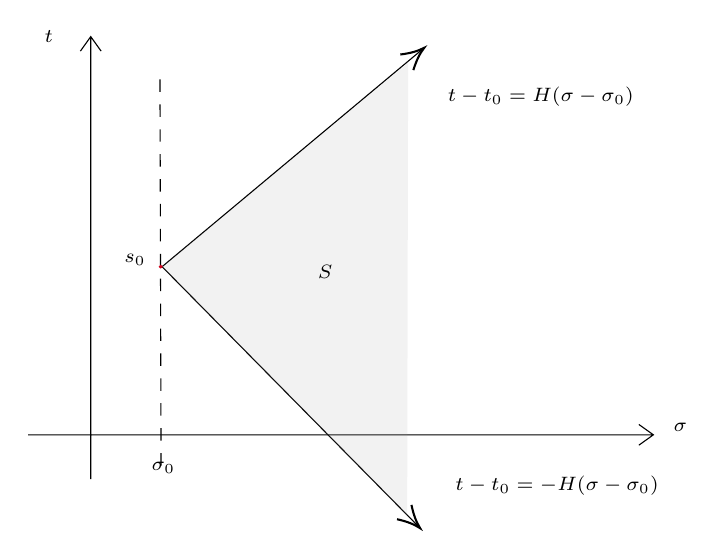
\begin{tikzpicture}[x=0.75pt,y=0.75pt,yscale=-1,xscale=1]
%uncomment if require: \path (0,300); %set diagram left start at 0, and has height of 300

%Shape: Axis 2D [id:dp1346371884561901] 
\draw  (151.5,207.43) -- (452.69,207.43)(181.62,15.58) -- (181.62,228.75) (445.69,202.43) -- (452.69,207.43) -- (445.69,212.43) (176.62,22.58) -- (181.62,15.58) -- (186.62,22.58)  ;
%Straight Lines [id:da6627378326231086] 
\draw  [dash pattern={on 4.5pt off 4.5pt}]  (214.97,36.22) -- (215.5,222.86) ;
%Straight Lines [id:da15935893462766404] 
\draw    (216,126.43) -- (338.94,251.02) ;
\draw [shift={(340.34,252.44)}, rotate = 225.38] [color={rgb, 255:red, 0; green, 0; blue, 0 }  ][line width=0.75]    (10.93,-4.9) .. controls (6.95,-2.3) and (3.31,-0.67) .. (0,0) .. controls (3.31,0.67) and (6.95,2.3) .. (10.93,4.9)   ;
%Straight Lines [id:da1539498165538844] 
\draw    (216,126.43) -- (340.78,22.23) ;
\draw [shift={(342.31,20.95)}, rotate = 140.14] [color={rgb, 255:red, 0; green, 0; blue, 0 }  ][line width=0.75]    (10.93,-4.9) .. controls (6.95,-2.3) and (3.31,-0.67) .. (0,0) .. controls (3.31,0.67) and (6.95,2.3) .. (10.93,4.9)   ;
%Shape: Ellipse [id:dp5156478132048201] 
\draw  [color={rgb, 255:red, 208; green, 2; blue, 27 }  ,draw opacity=1 ][fill={rgb, 255:red, 208; green, 2; blue, 27 }  ,fill opacity=1 ] (214.69,126.43) .. controls (214.69,126.1) and (214.98,125.83) .. (215.34,125.83) .. controls (215.71,125.83) and (216,126.1) .. (216,126.43) .. controls (216,126.76) and (215.71,127.03) .. (215.34,127.03) .. controls (214.98,127.03) and (214.69,126.76) .. (214.69,126.43) -- cycle ;
%Shape: Right Triangle [id:dp5295703844975419] 
\draw  [draw opacity=0][fill={rgb, 255:red, 155; green, 155; blue, 155 }  ,fill opacity=0.13 ] (334.53,28.25) -- (334.07,246.3) -- (216.03,126.43) -- cycle ;

% Text Node
\draw (158.18,11.54) node [anchor=north west][inner sep=0.75pt]  [font=\scriptsize]  {$t$};
% Text Node
\draw (461.16,200.54) node [anchor=north west][inner sep=0.75pt]  [font=\scriptsize]  {$\sigma $};
% Text Node
\draw (196.53,119.36) node [anchor=north west][inner sep=0.75pt]  [font=\scriptsize]  {$s_{0}$};
% Text Node
\draw (209.68,219.54) node [anchor=north west][inner sep=0.75pt]  [font=\scriptsize]  {$\sigma _{0}$};
% Text Node
\draw (352.39,38.8) node [anchor=north west][inner sep=0.75pt]  [font=\scriptsize]  {$t-t_{0} =H( \sigma -\sigma _{0})$};
% Text Node
\draw (356.09,225.92) node [anchor=north west][inner sep=0.75pt]  [font=\scriptsize]  {$t-t_{0} =-H( \sigma -\sigma _{0})$};
% Text Node
\draw (289.76,124.58) node [anchor=north west][inner sep=0.75pt]  [font=\scriptsize]  {$S$};


\end{tikzpicture}
\end{center}

\begin{proof}
Sean $H>0$, $\varepsilon>0$ dado y $1<M<N$, como la serie converge en $s=s_0$, entonces:

$$\sum_{M<n \leq N} f(n) n^{-s_0} n^{s_0-s}=\int_M^N t^{s_0-s} d A(t)=\int_M^N t^{s_0-s} d(A(t)-A(M))$$

Con $A(t)=\displaystyle\sum_{n \leq t} f(n) n^{-s_0}$, luego:
$$
\begin{aligned}
\sum_{M<n \leq N} f(n) n^{-s} & =\frac{A(N)-A(M)}{N^{s-s_0}}- \int_M^N(A(t)-A(M)) d(t^{s_0-s})\\
&=\frac{A(N)-A(M)}{N^{s-s_0}}-(s_0-s)\int_M^N(A(t)-A(M))t^{s_0-s-1}dt
\end{aligned}
$$

Tenemos que $A(t)$ converge cuando $t\to\infty$, luego $A(N)-A(M)$ y $A(t)-A(M)$ convergen a 0 cuando $M,N\to \infty$. Así, para $M, N$ suficientemente grandes y $\sigma>\sigma_0$:

$$|A(N)-A(M)|<\frac{\varepsilon}{(H+2)}, \quad|A(t)-A(M)|<\frac{\varepsilon}{H+2}$$

De esto se sigue que:

$$\begin{aligned}
\left|\sum_{M<n \leq N} \frac{f(n)}{n^s}\right|&<\frac{\varepsilon}{H+2}+\frac{\varepsilon}{H+2}\left|s-s_0\right| \int_M^{\infty} t^{\sigma_0-\sigma-1} d t\\
&=\frac{\varepsilon}{H+2}+\frac{\varepsilon\left|s-s_0\right|}{(H+2)\left(\sigma-\sigma_0\right) M^{\sigma-\sigma_0}}\\
&\leq\left(1+\frac{\left|s-s_0\right|}{\sigma-\sigma_0}\right) \frac{\varepsilon}{H+2} .
\end{aligned}$$

Queremos ver que $\left|\displaystyle\sum_{M<n \leq N} f(n) n^{-s}\right|<\varepsilon$, así el teorema se sigue de el teorema de Cauchy para convergencia uniforme de series, En efecto:

$$\left|s-s_0\right|=\left|\left(\sigma-\sigma_0\right)+i\left(t-t_0\right)\right| \leq \sigma-\sigma_0+\left|t-t_0\right| \leq\sigma-\sigma_0+H(\sigma-\sigma_0)\leq(H+1)\left(\sigma-\sigma_0\right)$$

Así:

$$\left|\sum_{M<n \leq N} \frac{f(n)}{n^s}\right|<(1+(H+1))\frac{\varepsilon}{H+2}=\epsilon$$
\end{proof}


Note que haciendo $H$ suficientemente grande obtenemos que $F(s)$ converge para todo  $s$ en el semiplano $\sigma>\sigma_0$, geométricamente lo que hacemos es abrir el cono de la región $S$ para obtener este semiplano.

\begin{theorem}
Supongamos que $F(s)=\displaystyle\sum_{n=1}^{\infty} f(n)n^{-s}$ no converge para todo $s\in \C$ ni diverge para todo $s\in\C$, entonces existe $\sigma_c\in \R$ tal que $F(s)$ converge para todo $s$ con $\sigma>\sigma_0$ y diverge para todo $\sigma<\sigma_0$.
\end{theorem}


\begin{proof}
Como mencionamos antes, tomando $H$ suficientemente grande vemos que si $F(s)$ converge en $s=s_0$, entonces por el teorema anterior $F(s)$ converge para todo $\sigma>\sigma_0$, por tanto, de manera análoga a la prueba del teorema 1.26, consideremos el conjunto:

$$A=\left\{a \in \mathbb{R} : \sum_{n=1}^{\infty} f(n) n^{-a} \text { converges }\right\}$$

Nuevamente  consideremos $\sigma_c$ el mínimo de $A$, si $s$ tiene parte real $\sigma>\sigma_c$, entonces $\sigma>a$ para algún $a\in A$, luego $F(s)$ converge, si $s$ tiene parte real $\sigma<\sigma_c$, entonces $\sigma<\dfrac{\sigma+\sigma_c}{2}<\sigma_c$ y como $\sigma_c$ es el mínimo, $\dfrac{\sigma+\sigma_c}{2}\not\in A$, lo que implica que $F(s)$ diverge.
\end{proof}
